\documentclass[compress]{beamer}

\usepackage[nofonts]{ctex}
\setCJKmainfont[ItalicFont={Kaiti SC}]{Kaiti SC}%
%\setCJKmainfont[ItalicFont={AR PL KaitiM GB}]{AR PL KaitiM GB}%
%\setCJKsansfont{WenQuanYi Zen Hei}% 文泉驿的黑体

\mode<beamer>
{
    \setbeamercovered{transparent}
    \useinnertheme{rounded}
    \useoutertheme{split}
    \usecolortheme{rose}
    \usecolortheme{seahorse}

	\expandafter\def\expandafter\insertshorttitle\expandafter{%
	\insertshorttitle\hfill%
	\insertframenumber\,/\,\inserttotalframenumber}
}

\mode<handout>
{
	\usetheme{default}
	\usepackage{pgfpages}
	\pgfpagesuselayout{4 on 1}[a4paper,landscape,border shrink=5mm]
}


\usepackage{amsmath,latexsym,amssymb,amsfonts,amsbsy}
\usepackage{graphicx}
\usepackage{hyperref}
\usepackage{fancyvrb}
\fvset{frame=single,fontsize=\small}

\newcommand{\romannumber}[1]{{\textrm{\uppercase\expandafter{\romannumeral
#1}}}}
\setbeamercolor{dblue}{fg=white,bg=blue!40!black} % for beamercolorbox
\newenvironment{pblock}{\begin{beamercolorbox}[rounded=true,
                                  shadow=true]{dblue}}{\end{beamercolorbox}}

\graphicspath{{figure/}}

%%%%%%%%%%%%%%%%%%%%%%%%%%%%%%%%%%%%%%%%%%%%%%%%%%%%%%%%%%%%%%%%%
%    body                                                       %
%%%%%%%%%%%%%%%%%%%%%%%%%%%%%%%%%%%%%%%%%%%%%%%%%%%%%%%%%%%%%%%%%


\begin{document}

\AtBeginSection[]
{ 
    \begin{frame}<beamer> 
		\frametitle{内容提要} 
		\tableofcontents[currentsection,currentsubsection] 
	\end{frame} 
} 
					
\title{协同开发工具}

\author[\href{http://c.pku.edu.cn/}{http://c.pku.edu.cn/}]
{曹东刚\\\href{mailto:caodg@sei.pku.edu.cn}{caodg@sei.pku.edu.cn}}

\institute{Linux程序设计环境 \\
\href{http://c.pku.edu.cn/}{
http://c.pku.edu.cn/}}

\date{}

\titlegraphic{
\includegraphics[height=0.17\textwidth]{Overlays/logo.pdf}}

\begin{frame}
	\titlepage
\end{frame}

\section{patch}

\begin{frame}
\frametitle{diff 和 patch}

\alert{diff} 和 \alert{patch} 是Unix的源码补丁工具

\begin{itemize}
\item \alert{diff} 以``行''为单位比较两个文本文件(也可以是目录比较),并将不同之处以某种格式输出到标准输出上;
\item \alert{patch} 可以读入这种输出, 并按照一定指令使源文件(目录)按照目标文件(目录)更新。
\end{itemize}

\end{frame}

\begin{frame}[containsverbatim]
\frametitle{diff}
diff用于生成源码补丁, 其命令格式为:\\[1ex]
{\small
\begin{Verbatim}

diff [命令行选项] 原始文件 新文件
常用命令行选项如下:
  -r 递归处理目录     
  -u 输出统一格式(unified format)
 -N patch里包含新文件
  -a patch里可以包含二进制文件
\end{Verbatim}
}

\alert{diff}的缺省输出在stdout上, 实际可能需要把它重定向到一个文件

\end{frame}

\begin{frame}
\frametitle{diff的输出格式}
diff的输出有``命令格式''和``上下文格式''几种, 现在大都使用上下文格式
\begin{itemize}
\item 命令模式分为两种:
    \begin{itemize}
    \item ed命令格式(缺省或--e选项)
    \item RCS(Revision Control System, 版本控制系统)命令格式(--n选项)
    \end{itemize}
\item 上下文模式也按格式分为两种
    \begin{itemize}
    \item 老版(--c 选项, 也称拷贝上下文)
    \item 新版(--u选项, 也称统一上下文)
    \end{itemize}
\end{itemize}

\end{frame}

\begin{frame}[containsverbatim]
\frametitle{命令格式}

缺省情况下\alert{diff}输出ed命令格式, 特点是简洁, 除了要删除/插入的行外没有冗余信息。\\
输出结果可以直接作为ed的命令控制文件\\[1ex]
\begin{Verbatim}
[caodg@debian]$ diff a.txt b.txt
1a2
> here we insert a new line
3d3
< why not this third line?
\end{Verbatim}

\end{frame}

\begin{frame}[containsverbatim]
\frametitle{上下文格式}

上下文格式保存了源文件上下文(缺省是上下各三
行), 同时在输出开头用\verb~---~和\verb~+++~标示出原始文件
和当前文件, 方便阅读\\[1ex]
{\small
\begin{Verbatim}
[caodg@debian]$ diff -u a.txt b.txt
--- a.txt Thu Apr 6 15:58:34 2000
+++ b.txt Thu Apr 6 15:57:53 2000
@@ -1,3 +1,3 @@
This is line one
+here we insert a new line
and this is line two
-why not this third line?
\end{Verbatim}
}

\end{frame}

\begin{frame}[containsverbatim]
\frametitle{patch}
\begin{itemize}
\item \alert{patch}命令把\alert{diff} 生成的补丁应用到现有代码上

\item \alert{patch}本身支持多种\alert{diff}输出文件格式

\item 对目标文件应用两次\alert{patch}, 则还原为原来的文件

\item 如果patch成功, 缺省不建备份文件

\item 如果patch失败, \alert{patch}会把成功的patch行给patch上同时(无条件)生成备份文件和一个.rej文件。
\end{itemize}

\alert{patch}常用选项: \\
\verb~    patch -p[patch level] < patchfile ~

\end{frame}

\begin{frame}[containsverbatim]
\frametitle{patch level}

\alert{diff}生成的patch文件里保存了目录路径, 通常如果当前目录树根目录和patch文件中的路径不一定匹配,
此时直接应用patch会失败.\\[1ex]
{\small
\begin{Verbatim}
diff -Nur p1/hello2.c p2/hello2.c
--- p1/hello2.c 2006-05-07 00:03:38.000000000 +0800
+++ p2/hello2.c 1970-01-01 08:00:00.000000000 +0800
\end{Verbatim}
}

patch level就是为解决该问题而设: patch会把目标路径名去掉开头patch level个目录
(由/分开的部分)
\begin{Verbatim}
cd p1
patch -p1 < ../patch.p
\end{Verbatim}

\end{frame}

\begin{frame}[containsverbatim]
\frametitle{应用diff和patch}

假定program-1.0目录中为老版, 现开发完成的新版位于program-2.0目录中, 
要将程序的1.0版本升级为2.0版本:
\begin{itemize}
\item 将两个目录置于同一父目录下, 在父目录生成patch: \\
  {\small \verb~diff -Nur program-1.0 program-2.0 > program-2.0.patch~ }
\item 其他开发者拿到patch后在自己的program-1.0目录执行:\\
\verb~patch -p1 < program-2.0.patch~
\item 如此即完成了从1.0到2.0的升级
\end{itemize}

\end{frame}

\section{版本控制}

\begin{frame}
\frametitle{什么是版本控制}
版本控制(Version control, 又称Revision control)是一种软件工程活动,
对软件配置项(Software configuration item: 程序, 文档及数据等)的变动进行管理。
\begin{itemize}
\item 最简单的版本控制就是手工保留软件不同版本的数份copy, 并且适当编号
    \begin{itemize}
    \item 效率低, 易错, 不适用于中大型项目, 不适用于多人协作开发
    \end{itemize}
\end{itemize}

\end{frame}

\begin{frame}
  \frametitle{为什么需要版本控制}
  \begin{itemize}
	\item 为整个项目提供Undo机制
	\item 帮助多个人同时修改同一个代码段
	\item 能记录所有的变动
	\item 支持多个发布版本,而不影响开发主线
	\item 可查看任何日期的项目状态
  \end{itemize}
\end{frame}

\begin{frame}
\frametitle{版本变动}

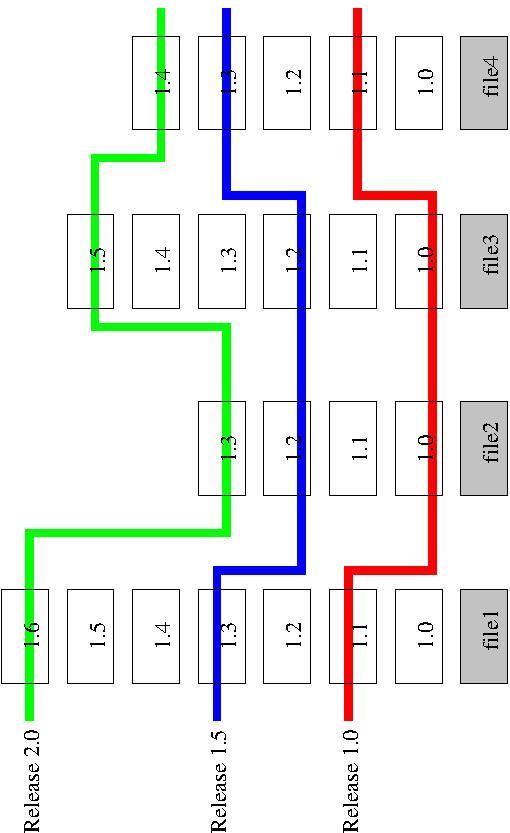
\includegraphics[angle=-90,width=\hsize]{revision.pdf}

\end{frame}

\begin{frame}
\frametitle{版本控制系统}

版本控制系统: 一组计算机程序, 用于自动维护软件配置项的所有版本, 记录一个软件配置项的版本变更历史,
即已做变更的内容、变更日期、变更人的姓名以及变更的原因等

\begin{itemize}
\item 源码控制系统 (Source Code Control System, SCCS)
\item 修订控制系统 (Revision Control System, RCS)
\item 并发版本系统 (Concurrent Version System, CVS)
\item CVS替代系统 (Subversion, SVN)
\item 分布式版本控制系统 (GIT)
\end{itemize}
\end{frame}

\begin{frame}
\frametitle{版本控制系统主要功能}

\begin{itemize}
\item 保存任意一个软件配置项的版本变更历史
\item 当两个用户同时修改一个文件时, 尽可能地自动合并修改; 在不能合并时,给出提示
\item 比较不同版本之间的差异
\item 可以回退到所保存的源代码的任意版本
\item 可以创建代码分支, 便于软件并行开发和维护; 代码分支可以合并
\item 对软件配置项进行标记, 方便日后审查
\item 阻止未经授权的修改和查阅
\end{itemize}

\end{frame}

\begin{frame}
\frametitle{版本控制系统工作原理}
\begin{itemize}
\item 大部分的版本控制软件采用增量存储方式: 只保留档案各版本之间的差异
\item 传统上版本控制系统都是采用集中模式: 所有版本控制的工作在一个服务器进
行, 程序员从服务器存储库(repository)签出(checkout)代码副本到本地工作空间, 在本地修改后提交(commit)到服务器
\item 2000年后, TeamWare, BitKeeper, 和GNU开始用分布式系统: 在分布式系
统中开发者直接在各自的本地存储库工作,各个存储库之间可以分享变更
\end{itemize}

\end{frame}

\begin{frame}
\frametitle{集中式版本控制系统}
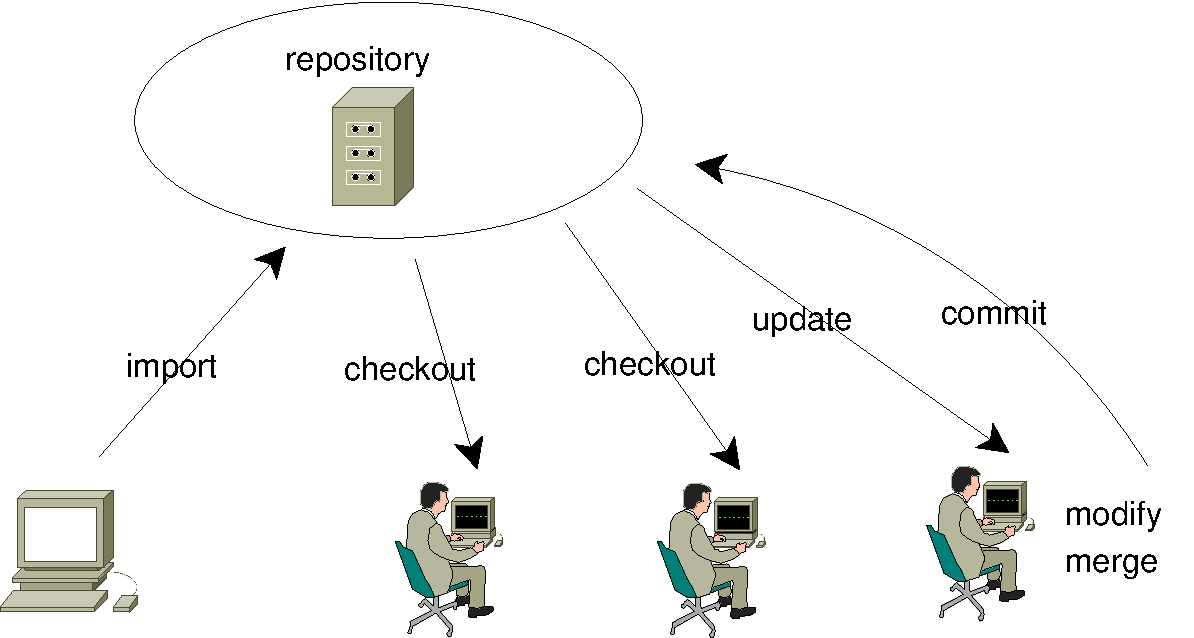
\includegraphics[width=\hsize]{centralized.pdf}

\end{frame}

\begin{frame}
  \frametitle{什么应该由版本控制系统管理}
  \begin{itemize}
	\item 源程序
	\item Makefile或build.xml
	\item 元数据
	\item 用于打包、测试、发布等的脚本文件
  \end{itemize}
  判断原则: 如果不维护文件$x$的状态, 项目就不能编译、发布, 
  那么$x$应该放入版本控制系统
  
\end{frame}

\begin{frame}
\frametitle{关键术语--1}
\begin{itemize}
\item 存储库(repository): 保存所有软件配置项的完整修订历史的共享数据库, 
  位于服务器侧
\item 工作空间(workspace): 要在本地编辑的文件副本. 
  在工作空间中编辑文件后要将更改返回存储库, 以便其他人可以看到这些更改
  \end{itemize}

  
\end{frame}


\begin{frame}
\frametitle{关键术语--2}
\begin{itemize}
  \item 主干(trunk): 当前的主版本
  \item 标记(tag): 用于标识文件集合的编号方案, 可在某个时间点标记并命名这些文件集
  \item 分支(branch): 和主干并行的版本
  \item 修订版本号(revision number): 版本控制系统标记各个文件更新的编号. 
  每次编辑文件并将它提交回存储库时, 该文件的修订版本号将会自动增加
\end{itemize}


\end{frame}

\begin{frame}
\frametitle{关键术语--3}
\begin{itemize}
\item 导入(import): 将某一个项目(项目根目录)导入版本控制系统, 
  对之进行版本控制
\item 签出(checkout): 从存储库中将文件的最新修订版本复制到工作空间. 
  签出目录时,将签出该目录下的所有文件和子目录。
\end{itemize}

\end{frame}


\begin{frame}
\frametitle{关键术语--4}
\begin{itemize}
\item 提交(commit): 将更改后的工作副本返回存储库
\item 更新(update): 使工作副本与存储库同步。用户进行修改前, 应进行更新
\item 冲突(conflict): 当两名开发人员对同一文件的工作副本进行更改并提交时, 
  他们的工作可能会发生冲突
\item 合并(merge): 将对相同文件的不同工作副本进行的多个更改合并到存储库中

\end{itemize}

\end{frame}

\begin{frame}[containsverbatim]
\frametitle{RCS}
RCS是目前Unix世界最广泛应用的版本控制系统, 非常适合一个人或小型团队开发的项目

\begin{itemize}
\item 在当前目录下创建RCS目录: \verb~mkdir RCS~
\item 将文件导入RCS: \verb~ci filename~
\item 从RCS导出文件: \verb~co filename~
\item 将修改后的文件保存回RCS: \verb~ci filename~
\item 查看log: \verb~rlog filename~
\end{itemize}


\end{frame}


\begin{frame}
\frametitle{CVS}
\begin{itemize}
\item CVS于1990年代初期开发, 在开源社区得到广泛应用
\item CVS最初架构于RCS系统之上, 作为RCS的前端. 目前CVS完全和RCS独立
\item CVS适用于大中型项目的分布式开发
  \end{itemize}

  
\end{frame}

\begin{frame}
\frametitle{CVS的锁定机制}
\begin{itemize}
\item CVS在文件被签出(checkout)后, 并不对文件进行锁定; 而是在文件被提交(commit)时检查冲突, 并要求人工干预
    \begin{itemize}
    \item 发生冲突的几率实际上非常小
    \item 避免了``单人失效问题''(single person point of failure)
    \end{itemize}
\end{itemize}


\end{frame}

\begin{frame}[containsverbatim]
\frametitle{CVS基本操作--1}
\begin{itemize}
\item 客户端设置环境变量\\
\verb~CVSROOT=/var/cvsroot~\\
或者\\
{\small \verb~CVSROOT=:pserver:username@162.105.81.88:/var/cvsroot~}
\item 登录CVS服务器\\
\verb~cvs login~
\item 在CVS服务器上创建一个项目(把当前目录导入服务器)\\
\verb~cd $HOME/project_dir~\\
\verb~cvs import project_dir V1_0 R1_0~
\end{itemize}


\end{frame}

\begin{frame}[containsverbatim]
\frametitle{CVS基本操作--2}
\begin{itemize}
\item 签出工作副本到本地\\
\verb~cvs checkout project_dir~\\
此时可以对该副本进行修改
\item 提交修改: 对工作副本做的任意改动(增删改除)都要提交后才会在服务器生效\\
\verb~cvs commit~
\item 增加一个文件\\
\verb~cvs add [-kb] filename~\\
\verb~cvs commit~ \\
增加一个二进制文件要用\verb~-kb~选项.\\

\end{itemize}


\end{frame}

\begin{frame}[containsverbatim]
\frametitle{CVS基本操作--3}
\begin{itemize}
\item 同步本地工作副本和服务器的内容\\
\verb~cvs update~\\
在每天工作前和工作之后commit之前都应当update,以
保证本地代码总是最新的,且和服务器的代码无冲突。
\item 从项目中删除文件. 删除时, 应当先将某个源文件物理删除后, 再使用remove命令\\
\verb~rm file_name~\\
\verb~cvs remove file_name~\\
\verb~cvs commit~


\end{itemize}


\end{frame}

\begin{frame}[containsverbatim]
\frametitle{CVS基本操作--4}
\begin{itemize}
\item 查看修改历史\\
\verb~cvs log file_name~
\item 查看文件不同版本的区别\\
\verb~cvs diff -r1.3 -r1.5 file_name~\\
查看1.3版本与1.5版本的区别\\
\verb~cvs diff file_name~\\
查看本地和库中最新版本文件的区别

\item 标记版本号\\
\verb~cvs tag release_version~

\end{itemize}


\end{frame}


\begin{frame}
\frametitle{CVS缺点}

\begin{itemize}
\item 不支持对目录的版本管理
\item 不支持文件改名
\item 对二进制文件的支持不够
\item 分支功能难以使用
\item 标记功能效率低下
\end{itemize}

\end{frame}

\begin{frame}
\frametitle{Subversion}
继承了CVS的优点, 克服了其缺点:
\begin{itemize}
\item CVS的大多数特征
\item 目录, 改名, 文件元信息的版本管理
\item 原子提交
\item 分支、标记、合并操作非常容易
\item Apache通过WebDAV/DeltaV协议直接支持
\end{itemize}


\end{frame}

\begin{frame}[containsverbatim]

\frametitle{subversion基本用法}

{\small
\begin{Verbatim}
建立代码库    svnadmin create /path/to/repos
导入数据      svn import
签出数据      svn checkout
提交更新      svn commit filename
添加文件      svn add
删除文件      svn delele
复制文件      svn copy
移动文件      svn move
查询状态      svn status
检查不同      svn diff
同步工作目录  svn update
合并代码      svn merge;svn resolve
\end{Verbatim}
}
\end{frame}

\begin{frame}
  \frametitle{代码库的组织}
  假定repos是SVN的代码库, pkuas是repos下面的一个项目, pkuas的
  根目录组织:
  \begin{itemize}
	\item trunk
	\item branches
	  \begin{itemize}
		\item RB-1.0
		\item BUG-3051
		\item TRY-new-xml
	  \end{itemize}
	\item tags
	  \begin{itemize}
		\item REL-1.0
	  \end{itemize}
  \end{itemize}
  
\end{frame}

\begin{frame}
  \frametitle{branch和tag}
  \begin{itemize}
	\item branch是独立的分支, 可进行bug修订等
	\item tag只是某个特殊时间点项目的快照, tag通常只读
  \end{itemize}

  \centering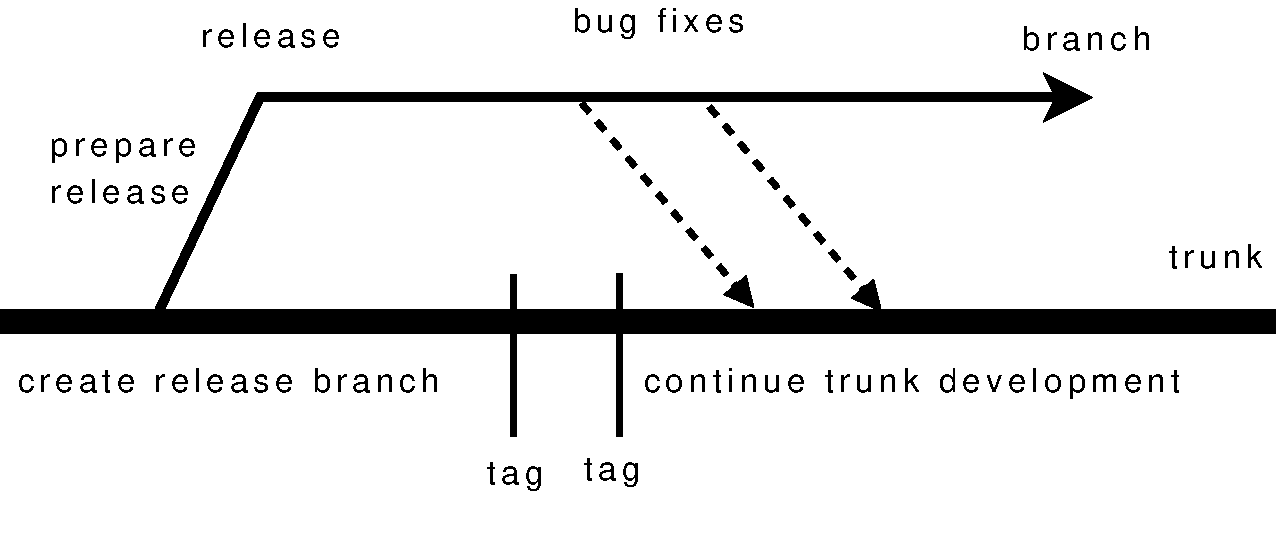
\includegraphics[width=\hsize]{branch.pdf}
  
\end{frame}

\begin{frame}[containsverbatim]
  \frametitle{创建和签出branch}
创建\\
  {\small
\begin{Verbatim}
work> svn copy -m "Creating release branch for 1.0" \
svn://olio/sesame/trunk \
svn://olio/sesame/branches/RB-1.0
Committed revision 33.
\end{Verbatim}
}
签出
{\small
\begin{Verbatim}
work> svn co svn://olio/sesame/branches/RB-1.0 rb1.0
A rb1.0/Month.txt
A rb1.0/common
A rb1.0/common/Log.java
Checked out revision 33.
\end{Verbatim}
}
  
\end{frame}

\begin{frame}[containsverbatim]
  \frametitle{在版本间切换}
{\small
\begin{Verbatim}
work> cd sesame
sesame> svn switch svn://olio/sesame/branches/RB-1.0
U common/Clock.java
U contacts/Contacts.java
Updated to revision 36.

sesame> svn switch svn://olio/sesame/trunk
U common/Clock.java
U contacts/Contacts.java
Updated to revision 36.
\end{Verbatim}
}
  
\end{frame}

\begin{frame}
    \frametitle{git}
    分布式的版本管理系统, 具有许多subversion不具备的优点
    \begin{itemize}
        \item 版本库是分布式的
            \begin{itemize}
                \item 每个人都可以拥有一个自己的版本库
                \item 提取操作实际上是一次对代码仓库的完整备份
                \item commit永远都会成功
                \item 可以离线提交
                \item 分支管理极其简单, 不同用户彼此不干涉
            \end{itemize}
        \item 版本库之间通过pull和push同步
        \item 速度快
        \item 可模拟subversion
    \end{itemize}
\end{frame}

\section{问题跟踪系统}

\begin{frame}
    \frametitle{Issue Tracking System}

\begin{block}{问题跟踪系统: ITS}
是专门用于记录、跟踪和管理各种问题的软件.\\
一贯地使用问题跟踪系统是优秀软件团队的标志特征之一
\end{block}

\begin{block}{问题: Issue}
对系统做出改进所需的一个工作单元. 典型的问题有: 缺陷(Bug), 任务(Task),
请求(Request Feature), 等.
\end{block}

\begin{block}{任务单: Ticket}
对于问题的技术性描述单位.
\end{block}
\end{frame}

\begin{frame}
    \frametitle{典型的问题处理流程}
    \begin{enumerate}
        \item 用户发现问题, 创建新ticket
        \item 管理员如果验证该问题合法,
            则转到\textcircled{\ref{ticket:valid}}; 否则 转到
            \textcircled{\ref{ticket:invalid}}
        \item \label{ticket:valid}确定负责解决该问题的技术人员
        \item 技术人员选择接受该ticket
        \item 技术人员解决该问题后, 打开该ticket, 描述如何解决的
        \item 用户收到关于该问题的解决情况的通知
        \item \label{ticket:invalid}项目管理员关闭该问题
    \end{enumerate}
\end{frame}

\begin{frame}[containsverbatim]
    \frametitle{Trac的Ticket}
    \begin{itemize}
        \item ID: 在wiki中通过 \verb~#num~ 直接引用
        \item 概述:对问题的一句话概要性描述
        \item 描述:对该问题的具体描述信息。应可重现
        \item 类型: 是Bug, Task, Enhancement
        \item 优先级: Critical, Major, Minor, Trivial
        \item 版本-构件: 发生该问题的具体版本-构件
        \item 里程碑: 什么时候该问题应该被解决
        \item 报告者: 提交问题的人
        \item 属主: 谁应该解决该问题
        \item 抄送: 谁应该关注该问题
    \end{itemize}
\end{frame}


\begin{frame}
    \frametitle{Trac的处理流程图}
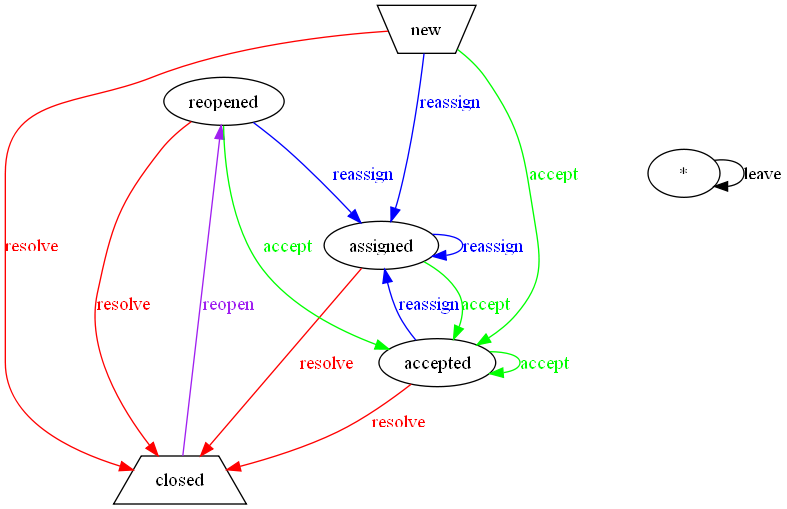
\includegraphics[width=\hsize]{basic-workflow.png}
\end{frame}

\begin{frame}
    \frametitle{问题驱动的开发}
    \begin{itemize}
        \item 规划项目的组成构件、项目的各个里程碑、版本
        \item 分解各个里程碑需要完成的任务, 并将任务分配到具体的程序员
            \begin{itemize}
                \item 任务必须是非常明确的、可执行、可测试的
                \item 关键任务应有单元测试用例
            \end{itemize}
        \item 里程碑的所有任务完成后, 应该进行一次版本发布,
            并提供该版本对系统的改动(ChangeLog), 这通常可自动生成
        \item 提交到代码库时,在提交说明中应标记此次提交对应的问题

        \item 每个里程碑应有集成测试用例
    \end{itemize} 
\end{frame}

\begin{frame}
    \frametitle{常见问题跟踪系统}
    \begin{itemize}
        \item Trac
        \item Redmine
        \item Bugzilla
        \item Launchpad
        \item Bugfree
        \item JIRA
        \item \dots
    \end{itemize}
\end{frame}

\section{Daily Build}

\begin{frame}
  \frametitle{Daily Build}
   每日创建: Daily build, nightly build
   \begin{enumerate}
	 \item 将一个软件项目的所有最新代码取出
	 \item 从头开始编译,链接
	 \item 生成文档、网页、发布包等
	 \item 运行测试软件包进行单元测试并对主要功能进行测试
	 \item 发现错误并报告错误
   \end{enumerate}
   上述过程完全自动化!
   
\end{frame}

\begin{frame}
  \frametitle{Daily build的好处}
  \begin{itemize}
	\item 及早发现不正确的代码提交
	\item 及早发现项目中存在的问题
	\item 对所有的变动进行自动化测试
	\item 随时可得到可运行的系统
	\item 减少风险
  \end{itemize}
\end{frame}

\begin{frame}
  \frametitle{如何进行 Daily build}
  需要有若干工具支持
  \begin{itemize}
	\item 源码控制系统: cvs, svn
	\item 编译工具: make(Makefile), ant(build.xml), maven
	\item 测试工具: Junit, Nunit
	\item 编译、运行、测试脚本
  \end{itemize}
\end{frame}

\begin{frame}
  \frametitle{利用 Unix 脚本进行Daily build}
  可以写一个Unix 脚本build.sh, 完成简单的daily build 功能
  \begin{itemize}
	\item 从cvs或svn中签出代码
	\item 调用make或ant进行自动编译
	\item 若有单元测试用例, 执行单元测试
	\item 上述任何步骤有错误都将错误信息通过email发送给项目组所有人
	\item 利用\alert{cron}设定系统在每日某个时刻自动调用build.sh脚本
  \end{itemize}
  
\end{frame}

\begin{frame}
  \frametitle{你有更多期望\dots}
  build.sh脚本能力相对局限. 你可能希望 
  \begin{itemize}
	\item 每次有程序员提交了代码, 都自动触发build脚本
	\item 在项目网页上生成自动build的统计信息, 
	\item 如果自动 build出错, 可以
	  \begin{itemize}
		\item 给你的手机、告警设备等发信息
		\item 定位错误源, 回退到上一个正确版本
		\item 和Bug管理系统集成
	  \end{itemize}
  \end{itemize}
 持续集成的概念
  
\end{frame}

\begin{frame}
  \frametitle{持续集成}
  持续集成(Continual Integration)是一种软件工程实践, 
  是极限编程(Extreme Programming)中很重要的一种活动
  有若干持续集成工具:
  \begin{itemize}
	\item Cruise Control
	\item continuum
	\item bamboo(open source license) 
	\item hudson
	\item bitten
	\item buildbot
  \end{itemize}
\end{frame}


\end{document}
